%%%%%%%%%%%%%%%%%%%%%%%%%%%%%%%%%%%%%%%%%
% 
% LaTeX Template
% Version 3.1 (25/3/14)
%
%%%%%%%%%%%%%%%%%%%%%%%%%%%%%%%%%%%%%%%%%

%----------------------------------------------------------------------------------------
%	PACKAGES AND DOCUMENT CONFIGURATIONS
%----------------------------------------------------------------------------------------

\documentclass[12pt, a4 paper]{article}

\usepackage{tikz}
%\usepackage[top=2cm, bottom=2cm, outer=0cm, inner=0cm]{geometry}
\usepackage{graphicx} % Required for the inclusion of images
\usepackage{multicol} % Required for multicolumns
\usepackage{setspace} % Required for line spacing
\setlength\parindent{0pt} % Removes all indentation from paragraphs
\setlength{\columnseprule}{0.4pt} % Adds vertical line between multicolumns
\usepackage{multirow} % Required for multirows
\usepackage{booktabs} % For prettier tables
\usepackage{xcolor}
%\usepackage{tabularx}
%\renewcommand{\rmdefault}{ptm}

%\usepackage{helvet}

\usepackage{times} % Uncomment to use the Times New Roman font

%----------------------------------------------------------------------------------------
%	DOCUMENT INFORMATION
%----------------------------------------------------------------------------------------

\begin{document}

%\tikz[remember picture,overlay] \node[opacity=0.3,inner sep=0pt] at (current page.center){\includegraphics[width=\paperwidth,height=\paperheight]{placeholder.jpg}};

\clearpage

%\font\myfont=cmr12 at 35pt
%\title{\myfont  Event Name} % Write Event name here
%\author{}
%\date{\vspace{-10ex}}

%\maketitle % Insert the title, author and date
\setstretch{1.5}

%\tikz[remember picture,overlay] \node[opacity=0.8,inner sep=0pt] at (current page.center){
\includegraphics[width=\paperwidth,height=\paperheight]{Border48-A4--Arvin61r58.png}};
%\tikz[remember picture,overlay] \node[opacity=0.5,inner sep=0pt] at (current page.center){\includegraphics[width=\paperwidth,height=\paperheight]{color-2174049__340.png}};

\begin{center}
\Huge \bfseries \ttfamily SESSION ON APTITUDE AND PERSONALITY

DEVELOPMENT
\end{center}

\begin{center}
\large A Session on how to develope own personality 
\end{center}

\begin{center}
\begin{multicols}{2}
\begin{tabular}{l r}
Date: & 11/10/2018\\ % Date the event was held
Time: & 3:30 pm to 5:30 pm \\ % Time of event 
\end{tabular}
\columnbreak
\begin{tabular}{l r}
Venue: & Mechanical Seminar Hall  \\ % Venue of event
%Total Attendance: & Number \\ % Number of participants
\end{tabular}
\end{multicols}

\begin{Large}
\begin{multicols}{2}
A session on aptitude and personality development was organised on October 11,2018 from 3:30p.m. to 5:30 p.m. in mechanical seminar hall of the college. This session was organised to guide students about career related doubts in which field they should go after the completion of btech .

\columnbreak
%\includegraphics[width=\linewidth]{placeholder.jpg}
  %\caption{A boat.}
  %\label{fig:boat1}
\end{multicols}

\begin{multicols}{2}

%\includegraphics[width=\linewidth]{placeholder.jpg}

\columnbreak
The session was delivered by MUNISH DEWAN and session was hosted by 20 years + experienced IMS centre director to be hosted.

\end{multicols}

\newpage 

%\tikz[remember picture,overlay] \node[opacity=0.8,inner sep=0pt] at (current page.center){
\includegraphics[width=\paperwidth,height=\paperheight]{5TRrp44jc.png}};
%\tikz[remember picture,overlay] \node[opacity=0.8,inner sep=0pt] at (current page.center){\includegraphics[width=\paperwidth,height=\paperheight]{md_5b0912b7c0870.png}};

\begin{multicols}{2}
The free scholarship test was also conducted and winner was awarded with the Rs.2100.

\columnbreak
%\includegraphics[width=\linewidth]{placeholder.jpg}
  
\end{multicols}

\begin{multicols}{2}
%\includegraphics[width=\linewidth]{placeholder.jpg}

\columnbreak
The host cleared the doubts of student regarding which field they should choose after btech . Either they should go for GRE, BANK EXAMS, JOB or CAT. He explained the studentsabout the procedure of cat exams and how to prepare for it. They also mentioned that they guide students for various exams .
  
\end{multicols} 

\begin{multicols}{2}
He then wrapped the session by explaining that if you want to go in your core company then you should do mtech otherwise you should go with the mba.

\columnbreak
%\includegraphics[width=\linewidth]{placeholder.jpg}
  
\end{multicols} 

\begin{multicols}{2}
%\includegraphics[width=\linewidth]{placeholder.jpg}

\columnbreak
The session was very beneficial for the students who want to further continue with studies after completion of btech .
 

  
\end{multicols} 

\end{Large} 
\end{center}

\newpage 

%\tikz[remember picture,overlay] \node[opacity=0.8, inner sep=0pt] at (current page.center){
\includegraphics[width=\paperwidth,height=\paperheight]{5TRrp44jc.png}};
%\tikz[remember picture,overlay] \node[opacity=0.8,inner sep=0pt] at (current page.center){\includegraphics[width=\paperwidth,height=\paperheight]{md_5b0912b7c0870.png}};

\begin{center}
\Huge Pictures Section
\end{center}

\newpage 

\tikz[remember picture,overlay] \node[opacity=0.8,inner sep=0pt] at (current page.center){
\includegraphics[width=\paperwidth,height=\paperheight]{image1.jpeg}};

\newpage

\tikz[remember picture,overlay] \node[opacity=0.8,inner sep=0pt] at (current page.center){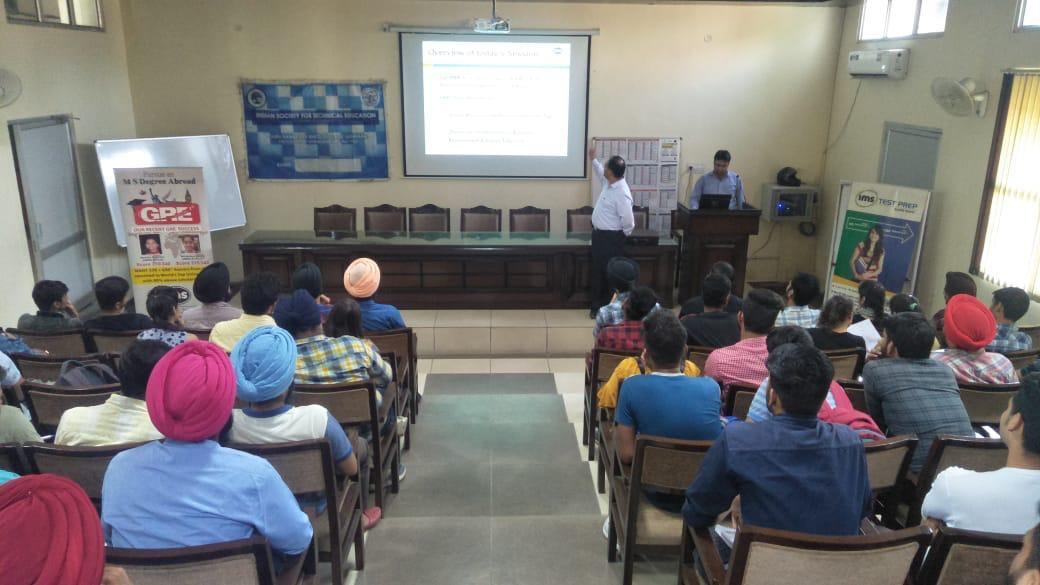
\includegraphics[width=\paperwidth,height=\paperheight]{image2.jpeg}};

\newpage

\tikz[remember picture,overlay] \node[opacity=0.8,inner sep=0pt] at (current page.center){
\includegraphics[width=\paperwidth,height=\paperheight]{image3.jpeg}};

\newpage

\begin{center}
\huge Organisers list
\end{center}

\begin{table}[h!]
  \begin{center}
    \begin{tabular}{|c|c|c|c|} 
    \toprule % <-- Toprule here
      \textbf{S.No.} & \textbf{Name} & \textbf{Branch/Year} & \textbf{Roll No.}\\
      \midrule % <-- Midrule here
      1 & Shubhendra & D2 CE & 1706310\\
      2 & Jagmeet Singh & D2 ECE & 1706728 \\
      3 & Tushar & D2 CSE & 1706533 \\
      4 & Kamya Arora & D2 CSE & 1706453 \\
      5 & Kavleen Kaur & D2 CSE & 1706457 \\
      6 & Parneet & D2 CSE & 1706486 \\
      7 & Sudhanshu & D2 CSE & 1706523 \\
      8 & Ishpreet Kaur & D2 CSE & 1706443 \\
      \bottomrule % <-- Bottomrule here
    \end{tabular}
  \end{center}
\end{table}


\newpage

\tikz[remember picture,overlay] \node[opacity=0.8,inner sep=0pt] at (current page.center){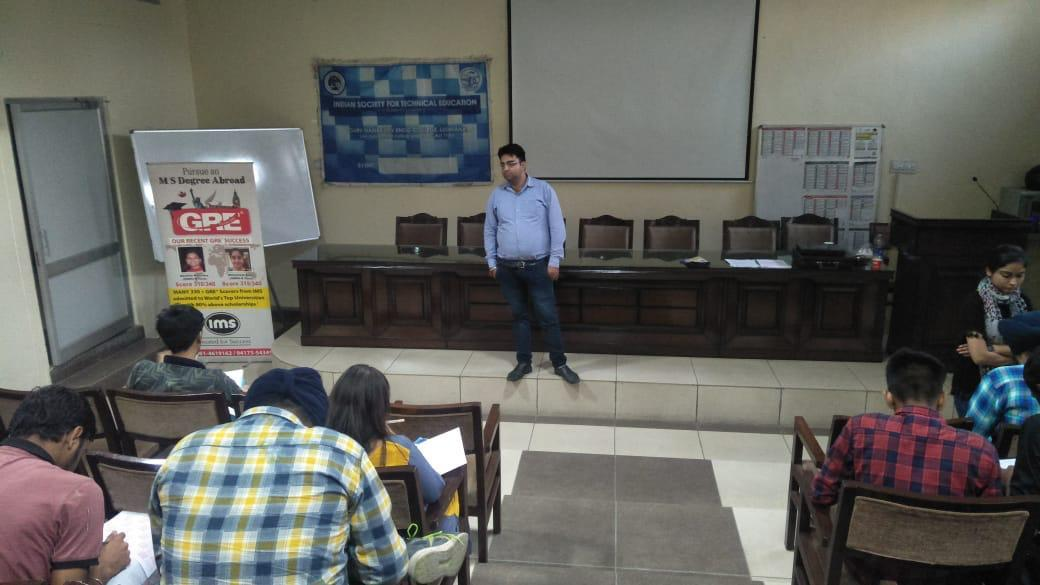
\includegraphics[width=\paperwidth,height=\paperheight]{image4.jpeg}};

\newpage

\tikz[remember picture,overlay] \node[opacity=0.8,inner sep=0pt] at (current page.center){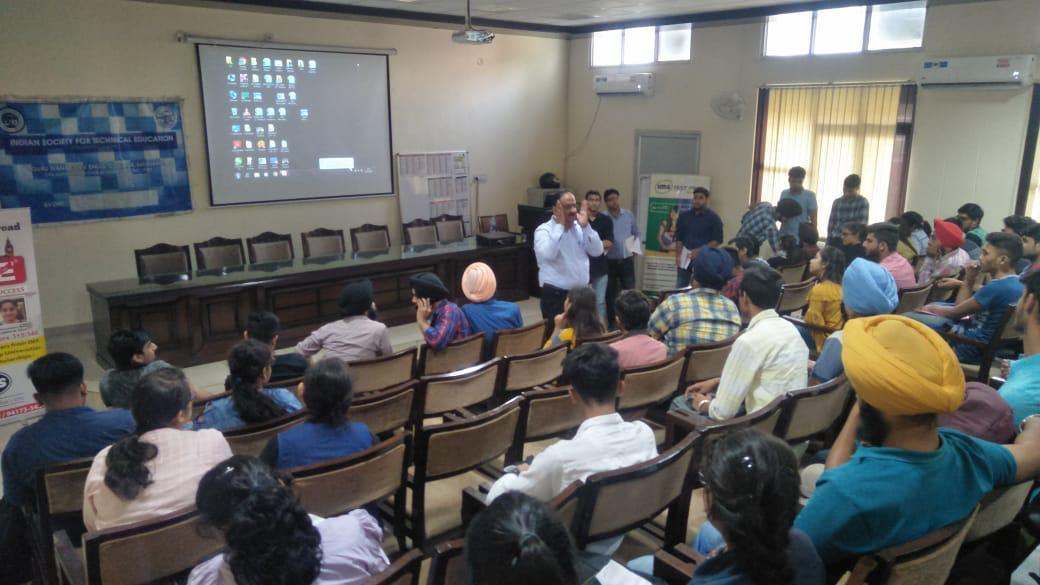
\includegraphics[width=\paperwidth,height=\paperheight]{image5.jpeg}};



\end{document}